\subsubsection{Llaves de activación modo aislado limitado y total}

El SAL/T permite la activación de los modos aislado limitado y modo aislado total de manera local. Para el modo aislado limitado, existe una llave colocada en el panel frontal del dispositivo que va a permitir la activación del modo. Para el modo aislado total, se coloca una llave por fuera del panel frontal, instalada dentro de algún lugar con acceso restringido al maquinista y solo accesible para el personal de mayor autoridad.  \\

La activación de estas llaves altera completamente el funcionamiento de la formación por lo que la correcta lectura de su estado es un requisito importante para el sistema. Por esto se eligió un modelo de llave interruptora bipolar de dos posiciones, ya que cuenta con dos líneas y permite medir el estado en dos entradas diferentes del MCU y asegurarse de leer la posición correcta. El modelo seleccionado es una llave interruptor Bipolar 20 A de dos posiciones de la empresa Elibet \cite{llave_elibet} que se puede visualizar en la figura \ref{fig:llave_mal} y está diseñada para ser colocada en un panel frontal. 

\begin{figure}[H]
    \centering
    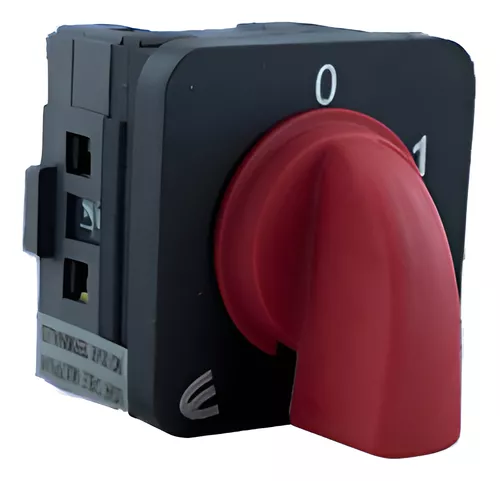
\includegraphics[width = 0.4\linewidth]{img/llave_mal.png}
    \caption{Llave interruptor bipolar 20A Elibet 0-1 posiciones}
    \label{fig:llave_mal}
\end{figure}

En la figura \ref{fig:llave_mal_sch} se muestra el circuito implementado para medir el estado de cada llave. Se conectaron resistencias de \textit{pull-up} de 40.2 k$\Omega$ y se conectaron las entradas de la llave a tierra. Cuando la llave está abierta, las señales que llegan al MCU, ON\_SW\_MAL\_1 y ON\_SW\_MAL\_2 quedan a 3,3 V y el MCU toma esos nodos como entradas digitales por lo que va a detectar un estado alto. Cuando la llave se cierra, los nodos quedan conectados a tierra y el MCU va a leer un estado bajo. En caso de inconsistencia entre los valores leídos entre las dos entradas de una misma llave, se considera el estado de no activación de la llave, ya que es el estado de mayor seguridad y no puede asegurarse el correcto funcionamiento del sistema sin una lectura correcta. 


\begin{figure}[H]
    \centering
    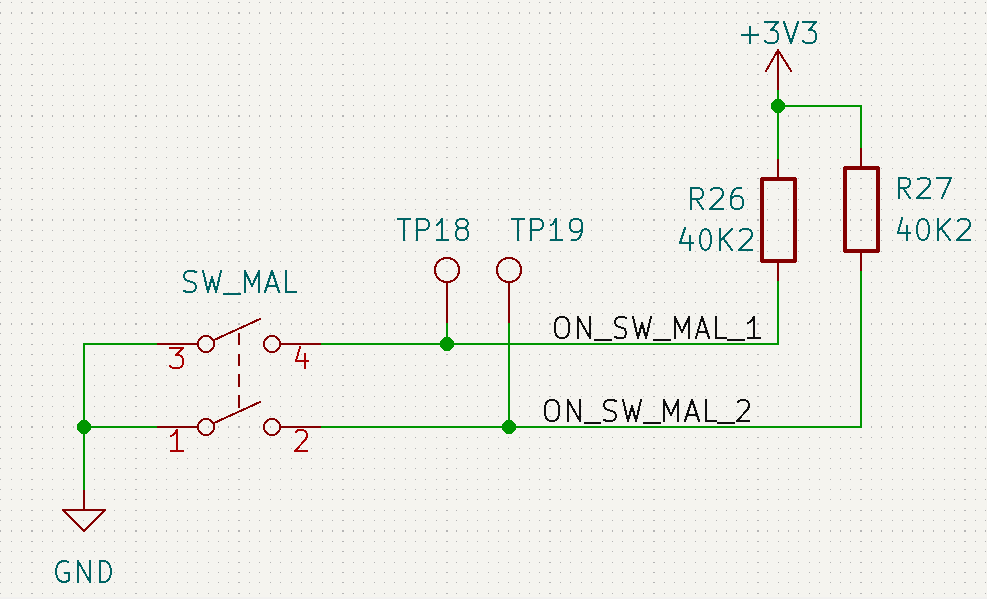
\includegraphics[width = 0.8 \linewidth]{img/llave_mal_sch.png}
    \caption{Circuito de lectura del estado de la llave interruptora}
    \label{fig:llave_mal_sch}
\end{figure}